\chapter{Kurze Darstellung der Theorie des Modellsupermarktes}
\label{chap:theorie}
\minitoc
In diesem Kapitel wird ein knapper Überblick über die mathematische und physikalische Zusammenhänge, die bei der Entwicklung eines
Modellsupermarktes zwingend beachtet werden müssen, vorgestellt\todo{Der Satz ist total scheiße man}. Es beinhaltet eine
Zusammenfassung des mathematischen Konstruktes aus dem Kapitel 3 der Diplomarbeit von Caroline Möller \cite{caro}, der bei der
Entwicklung des Programms zu Grunde gelegt wurde.

%%%%%%%%%%%%%%%%%%%%%%%%%%%%%%%%%%%%%%%%%%%%%%%%%%%%%%%%
%%%%%%%%%%%%%%%%%%%%%%%%%%%%%%%%%%%%%%%%%%%%%%%%%%%%%%%%
%%%%%%%%%%%%%%%%%%%%%%%%%%%%%%%%%%%%%%%%%%%%%%%%%%%%%%%%
\section{Ausformuliertes Einfügen}

Die primäre Aufgabe der Kühleinheiten in einem Supermarkt besteht in der Regel darin, Lebensmitteltemperatur unter die
Zimmertemperatur zu bringen und diese dabei zu halten\todo{Hört sich komisch an!}. Körper mit unterschiedlicher Temperatur
sind bestrebt, wenn sie thermisch von einander nicht vollkommen isoliert sind, durch gegenseitige Wechselwirkung ihre
Temperaturen anzugleichen, sodass ein Wärmegleichgewicht entsteht, wobei der natürliche, selbständige Wärmefluss immer von
einem Körper mit höheren Temperatur in Richtung des Körpers mit kleineren Temperatur stattfindet. Um eine negative
Temperaturänderung herzustellen und diese auch zu halten, muss die eindringende Wärmeenergie ständig in der selben Höhe
abgeführt werden, damit die Temperatur konstant bleibt. Diese Energiemenge pro Zeiteinheit wird als Kälteleistung bezeichnet.
Eine Abweichung von dieser Menge führt zum Steigen der Temperatur, wenn weniger und zum sinken der Temperatur wenn mehr
abgeführt wird. Um diesen Kühlkreislauf aufrecht zu erhalten, muss Leistung aufgewendet werden\footnote{ Eine detailierte
Beschreibung dieser Prozesse in einer Kopressionskälteanlage und Spezifikation ist nicht Gegenstand dieser Arbeit.
Ausführliche Informationen dazu findet man z.B.  in \cite{caro, doctor, TAB_A1}.}.


\subsection{Umsetzung der Ideen}
Die Bilder müssen hier eingefügt werden und mit UML Theorie erklärt werden, aber nicht viel.
\begin{figure}[h]
\caption{Klassendiagramm Modellkonstrukt}
	\label{klassendiagramm}
	\begin{center}
	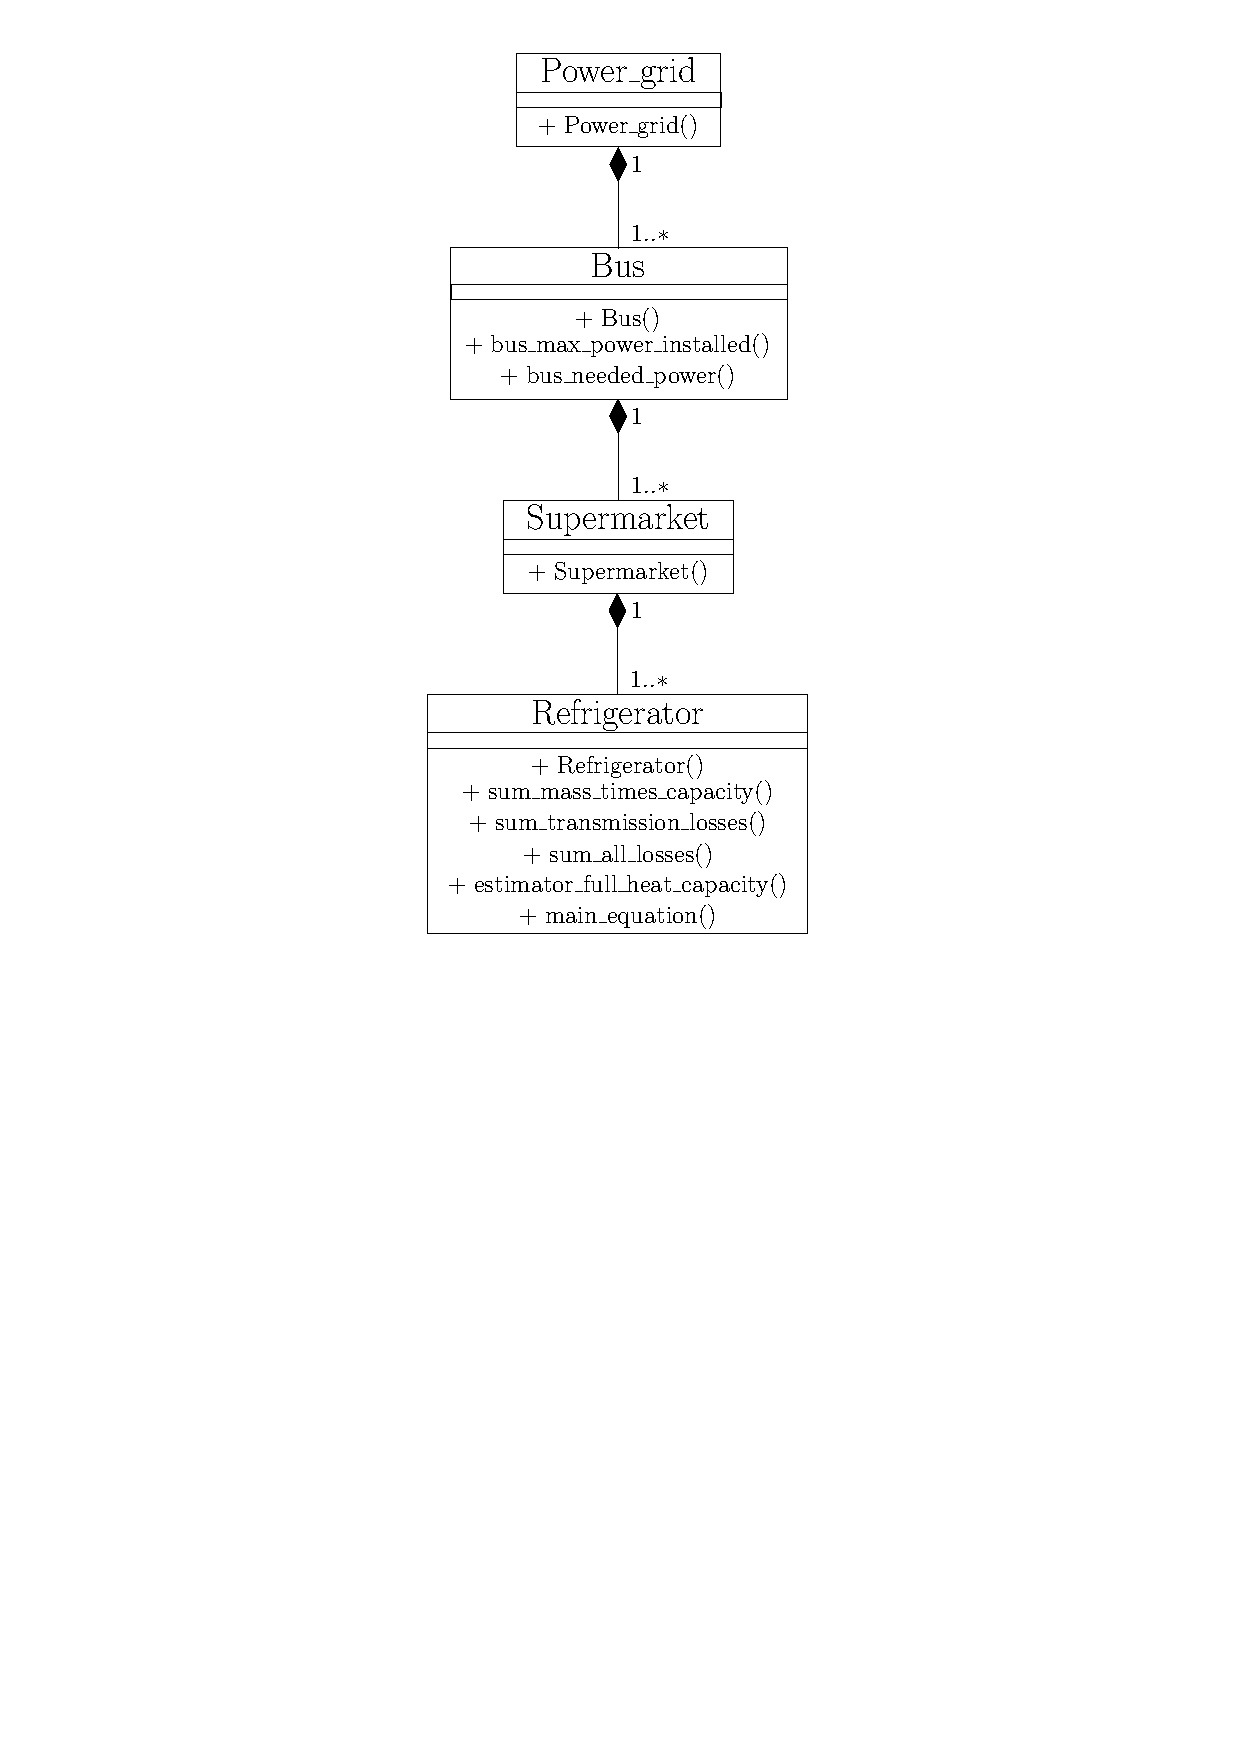
\includegraphics[scale=0.8]{images/Theorie_Super/class_diagramm}
	\end{center}
\end{figure}

Hier noch ein Zwischentext.

\begin{figure}[h]
\caption{Sequenzdiagramm Modellkonstrukt}
	\label{uml_sequence}
	\begin{center}
	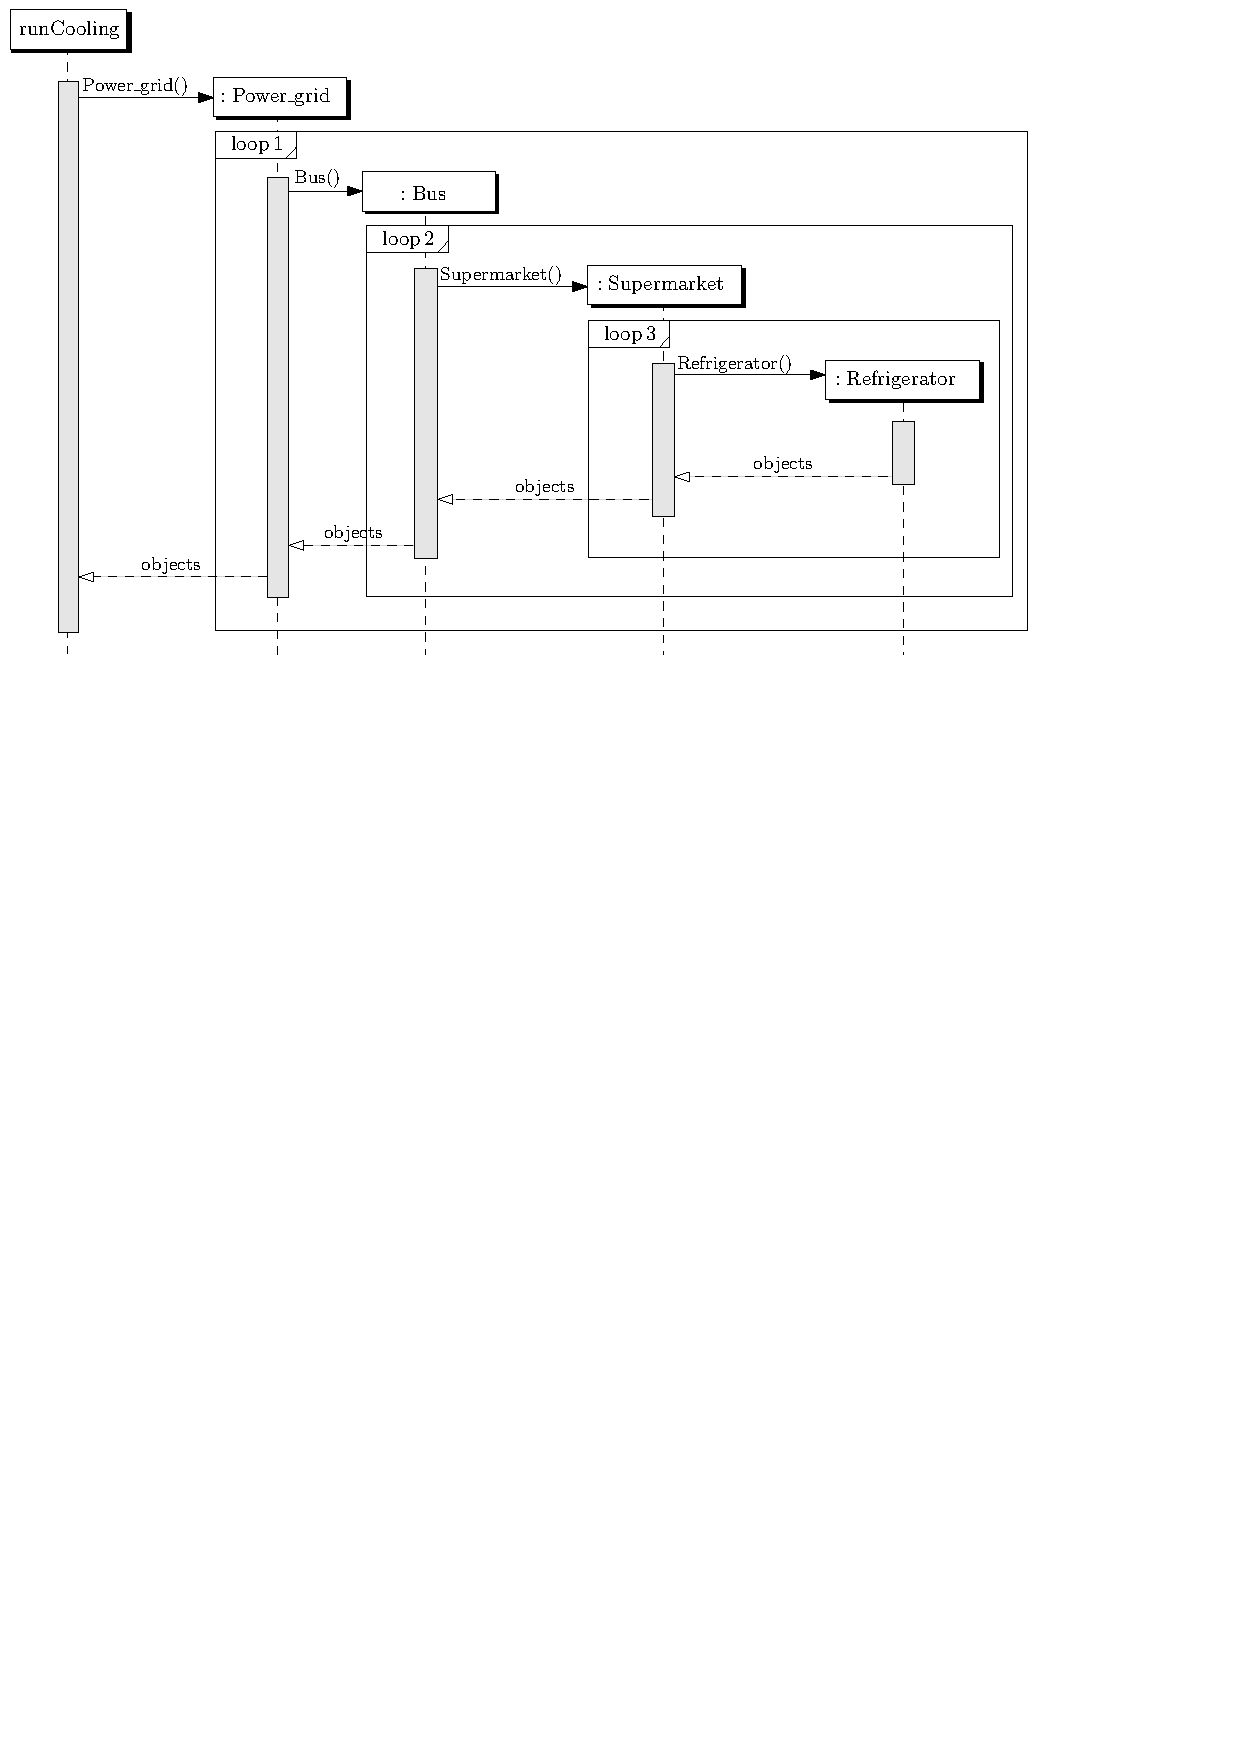
\includegraphics[scale=0.8]{images/Theorie_Super/sequence_one}
	\end{center}
\end{figure}
%\input{uml_sequence2}

%%%%%%%%%%%%%%%%%%%%%%%%%%%%%%%%%%%%%%%%%%%%%%%%%%%%%%%%
%%%%%%%%%%%%%%%%%%%%%%%%%%%%%%%%%%%%%%%%%%%%%%%%%%%%%%%%
%%%%%%%%%%%%%%%%%%%%%%%%%%%%%%%%%%%%%%%%%%%%%%%%%%%%%%%%
\section{Überblick über die mathematische Zusammenhänge}

Das wird ausformuliert und mit einem Bild visualisiert\todo{bald schnell machen}.
\begin{itemize}
	\item Temperaturunterschied
	\item Wärmeausgleich (Verlust an Kälte)
	\item Kälteenergie gespeichert in Körpern mit einer bestimmten spezifischen Wärmekapazität
	\item Kälteenergie gespeichert in Masse
\end{itemize}
\begin{figure}\caption{ Modellgrundlage}
	\missingfigure{Modellgrundlage}
\end{figure}

%%%%%%%%%%%%%%%%%%%%%%%%%%%%%%%%%%%%%%%%%%%%%%%%%%%%%%%%
%%%%%%%%%%%%%%%%%%%%%%%%%%%%%%%%%%%%%%%%%%%%%%%%%%%%%%%%
%%%%%%%%%%%%%%%%%%%%%%%%%%%%%%%%%%%%%%%%%%%%%%%%%%%%%%%%
\subsection{Wermeverlustquellen bei Kühlgeräten}

Die Temperaturdifferenz $\Delta\:t$ ist direkt proportional zur eindringenden Wärmeenergie $Q$ und wird mit
\begin{equation}
	\Delta t = \frac{Q}{m\cdot c}
\label{tdif}
\end{equation}
ermittelt, wobei $m$ die Masse des Stoffes, der die Wärmeenergie aufnimmt, und $c$ seine spezifische Wärmekapazität ist.
Wärmeverluste bedeuten hier die Verluste durch eindringende Wärme oder die „Verluste an Kälte“\cite{caro}.

%%%%%%%%%%%%%%%%%%%%%%%%%%%%%%%%%%%%%%%%%%%%%%%%%%%%%%%%
%%%%%%%%%%%%%%%%%%%%%%%%%%%%%%%%%%%%%%%%%%%%%%%%%%%%%%%%
%%%%%%%%%%%%%%%%%%%%%%%%%%%%%%%%%%%%%%%%%%%%%%%%%%%%%%%%
\subsection{Erforderliche Kälteleistung}

Gegeben sind also:
\begin{itemize}
	\item der Kältebedarf in \textit{kW} bei Kühlstellen, die zu einer Verbundanlage gehören,
	\item der elektrische Energieverbrauch in \textit{kWh$/24$ h} bei steckerfertigen Geräten,
	\item die installierte Verdichterkälteleistung in \textit{kW} bei Kälteaggregaten.
\end{itemize}
Die installierte Kälteleistung ist oft größer als der Kältebedarf. Bei Angaben zur installierten Kälteleistung muss deshalb
die tägliche Betriebszeit des Verdichters $\tau_B$ berücksichtigt werden. Die tägliche Betriebszeit des Verdichters ist in der
Literatur mit 16$h$ für Plusanlagen und 18$h$ für Minusanlagen angegeben. Unter Verwendung der Gleichung für die installierte
Kälteleistung $\pinstall$
\begin{equation}
	\pinstall = \frac{24}{\tau{B}} \label{pinstall}
\end{equation}
\noindent erhält man den Kältebedarf oder die erforderliche Kälteleistung $Q_0$ .

%%%%%%%%%%%%%%%%%%%%%%%%%%%%%%%%%%%%%%%%%%%%%%%%%%%%%%%%
%%%%%%%%%%%%%%%%%%%%%%%%%%%%%%%%%%%%%%%%%%%%%%%%%%%%%%%%
%%%%%%%%%%%%%%%%%%%%%%%%%%%%%%%%%%%%%%%%%%%%%%%%%%%%%%%%
\subsection{Transmissionswärmeleistung}

Die Wärmedurchgangskoeffizienten $k$, auch $k$-Werte genannt, welche angeben, wieviel Wärmeleistung pro $m^2$ und pro 1 $K$
Temperaturdifferenz durch die Wand diffundiert, sind wichtig für die Berechnung der Transmissionswärmeleistung $\ptrans$. Die
Transmissionswärmeleistung wird mit

\begin{equation}
	\ptrans = A \cdot k \cdot \Delta t \label{ptrans}
\end{equation}

\noindent berechnet, wobei $A$ die Fläche der wärmeübertragenden Wände und $\Delta \, t$ die Temperaturdifferenz der
Kühlraumtemperatur zur Umgebungstemperatur ist.

%%%%%%%%%%%%%%%%%%%%%%%%%%%%%%%%%%%%%%%%%%%%%%%%%%%%%%%%
%%%%%%%%%%%%%%%%%%%%%%%%%%%%%%%%%%%%%%%%%%%%%%%%%%%%%%%%
%%%%%%%%%%%%%%%%%%%%%%%%%%%%%%%%%%%%%%%%%%%%%%%%%%%%%%%%
\subsection{Leistungszahl}
\label{Leistungszahl}
Der Zusammenhang zwischen der aufgewendeten elektrischen Antriebsleistung eines Verdichters in einer Kompressionskälteanlage
$P$ und genutzten Kälteleistung ${\dot{Q}}_0$ wird durch die Kältezahl $\epsilon$ \cref{epsilon} wiedergegeben.

\begin{equation}
	\epsilon = \frac{\pkalt}{P}
\label{epsilon}
\end{equation}

\noindent Um auf die für die Kühlung in einer Stunde benötigte elektrische Leistung für eine Kühleinheit zu kommen, muss der
in dieser Stunde anfallende Bedarf an Kälteleistung durch die Leistungszahl dividiert werden. Die Leistungszahl wird in die
zweite Spalte im Array (vergl. Zeile 4 im \matref{fridge}) eingetragen.

%%%%%%%%%%%%%%%%%%%%%%%%%%%%%%%%%%%%%%%%%%%%%%%%%%%%%%%%
%%%%%%%%%%%%%%%%%%%%%%%%%%%%%%%%%%%%%%%%%%%%%%%%%%%%%%%%
%%%%%%%%%%%%%%%%%%%%%%%%%%%%%%%%%%%%%%%%%%%%%%%%%%%%%%%%
\subsection{Speichermittel, Kennzahl}

Neben den technischen Daten und den Abmaßen der Flächen, sind Angaben zur Art und Menge der eingelagerten Lebensmittel
notwendig. Deren Massen und spezifische Wärmekapazitäten sind ein wichtiges Kriterium für die Wärmespeicherfähigkeit und
damit den Temperaturverlauf, von dem wiederum die Nutzung als Speicher abhängt. Das Produkt aus Masse $m$ und spezifischer
Wärmekapazität $c$ wird auch absolute Wärmekapazität $C$ genannt. Je größer die absolute Wärmekapazität $C$, umso mehr Wärme
kann ein Produkt speichern und umso langsamer steigt seine Temperatur (vgl. \cref{tdif} auf Seite ).

%%%%%%%%%%%%%%%%%%%%%%%%%%%%%%%%%%%%%%%%%%%%%%%%%%%%%%%%
%%%%%%%%%%%%%%%%%%%%%%%%%%%%%%%%%%%%%%%%%%%%%%%%%%%%%%%%
%%%%%%%%%%%%%%%%%%%%%%%%%%%%%%%%%%%%%%%%%%%%%%%%%%%%%%%%
\subsection{Verbrauch abhängig von der Öffnungszeit}

Die Wärmeverluste sind abhängig von den Öffnungszeiten des Supermarkts. In der Nacht, wenn der Markt geschlossen ist, werden
offene Kühlregale in nahezu allen Supermärkten mit Nachtrollos verschlossen. Die folgenden Rechnungen gehen davon aus, dass
Verluste in der Nacht bei geschlossenem Supermarkt nur durch Transmissionswärme auftreten. Die Beleuchtung ist ausgeschaltet,
die Türen werden nicht geöffnet, die offenen Kühlregale sind mit Nachtrollos verschlossen. Es gibt keine Personen im Markt, die
Wärme abgeben. Die Truhen können mit Nachtabdeckplatten aus Kunststoffschaum abgedeckt werden [COP-10]. Durch diese Maßnahmen
sinkt der Energieverbrauch auf 10 bis 20\% des Bedarfs während der Öffnungszeiten [KAU-08].

Am Tag müssen neben den Verlusten durch die Transmissionswärme auch alle anderen Verluste, die auftreten, berücksichtigt
werden. Diese zusätzlichen Verluste werden zur Vereinfachung als weitgehend konstant angenommen.
Aus den soeben angestellten Überlegungen folgt:

\begin{equation}
	\dot{Q}_{Nacht}=\ptrans
\label{pnacht}
\end{equation}
und
\begin{equation}
	\dot{Q}_{Tag} = \pmehr + \ptrans
\label{ptag}
\end{equation}

Für die Kälteverbraucher, bei denen der Kältebedarf gegeben ist, kann die \cref{ptag} unter Berücksichtigung von
$\dot{Q}_0 = \dot{Q}_{Tag}$  und des Faktors für die Kältebedarfsabsenkung $K$ zur Berechnung des Mehrbedarfs an Leistung
$\pmehr$ verwendet werden. Da für $\pmehr$ jedoch ein konstanter Wert gebraucht wird, muss auch mit einem konstantem Wert für
$\ptrans$ gerechnet werden. Dieser wird einmalig aus der mittleren Kühlraumtemperatur $\overline{t}_{KR}$ mit folgender Gleichung
gebildet und nur für die Berechnung von $\pmehr$ verwendet.

\begin{equation}
	\overline{\dot{Q}}_{Tr} = A \cdot k \cdot \left( t_{amp} - \overline{t}_{KR} \right)
\label{ptrans}
\end{equation}

Der Fehler, der durch diese Mittelung entsteht, ist vernachlässigbar, da die Transmissionswärmeverluste sehr gering sind im
Vergleich zu den Gesamtwärmeverlusten am Tag und diese aufgrund des gegebenen oder ermittelten Kälteleistungsbedarfs $Q_0$
konstant sind.

Folgender Ausdruck ergibt sich damit für $\pmehr$ bei Kälteverbrauchern mit gegebener Kälteleistung:
\begin{equation}
	\pmehr = \pkalt \cdot K - \overline{\dot{Q}}_{Tr}%
\label{pmehr}
\end{equation}

Aufgrund der nicht vorhandenen Angabe für den Kältebedarf bei steckerfertigen Geräten ist eine zweite Methode notwendig, um
auch hier den Mehrbedarf am Tag zu ermitteln. Der Wert des spezifischen elektrischen Energieverbrauchs pro 24 Stunden ist bei
diesen Geräten gegeben. Mit dieser Angabe kann wie folgt gerechnet werden. Zunächst wird der spezifische Energieverbrauch
$\lspez$ mit dem Faktor für die Kältebedarfsabsenkung $K$, dem Verdichteranteil $v$ und mit der Anzahl der Geräte $n$
multipliziert.  Als Ergebnis erhält man die Verdichterarbeit pro 24 Stunden $\lverd$ für den gesamten Kälteverbraucher.

\begin{equation}
	\lverd = \lspez \cdot K \cdot v \cdot n
\label{lverd}
\end{equation}

Werte für den Anteil der Verdichterarbeit am Gesamtenergieverbrauch sind in der Literatur mit 0,627 [PER-06] oder 0,66
[KAU-08] gegeben.  Der Anteil der Verdichterarbeit $\lmehr$, der zuständig ist für das Abführen der eindringenden Wärmeenergie
$\emehr$ ergibt sich mit folgender Gleichung:

\begin{equation}
	\lmehr = \lverd - \frac{\ptrans}{\epsilon} \cdot 24h \cdot
\label{lmehr}
\end{equation}

Die Wärmeleistung $\pmehr$ lässt sich dann anschließend mit
\begin{equation}
	\pmehr = \frac{\lmehr}{12h} \cdot \epsilon
\label{<++>}
\end{equation}
berechnen.

Dabei entspricht $\pnacht$ der mittleren Transmissionswärmeleistung $\ptrans$. $\ptag$ ist der Kältebedarf $\pkalt$,
multipliziert mit dem Faktor für die Kältebedarfsabsenkung $K$ bei Geräten, bei denen der Kältebedarf gegeben ist. Bei
steckerfertigen Geräten ist $\ptag$ die Summe aus dem Mehrbedarf an Leistung am Tag $\pmehr$ und der mittleren
Transmissionswärmeleistung $\ptrans$.

\subsection{Berechnung der Temperaturänderung}
Mit den Wärmeverlusten, die am Tag und in der Nacht in unterschiedlicher Größe auftreten, wird für jeden Zeitschritt die Zeit
bis zum kritischen Temperaturmaximum bestimmt. Diese Zeit braucht das Programm, um den Einsatz der Supermarktkälteanlagen als
Speicher zu planen. Mit der Gleichung
\begin{equation}
	\tau_{krit}(i) = \frac{m \cdot c \cdot (t_{max} - t(i))}{\overline{\dot{Q}}_{Tr_{ln}}}
\label{taukn}
\end{equation}
wird die Zeit $\tau_{krit}$ für jeden Zeitpunkt $i$ berechnet, wobei $\overline{\dot{Q}}_{Tr_{ln}}$ der logarithmische Mittelwert
ist, der sich aus den Transmissionswärmeleistungen zum jeweils aktuellen Zeitpunkt $i$ mit der Temperatur $t(i)$ und den
Transmissionswärmeleistungen zum Zeitpunkt, an dem der Kühlinnenraum die maximale Temperatur $t_{max}$ erreicht hätte,
berechnet. Am Tag müssen die restlichen Verluste $\pmehr$ zusätzlich zu den Transmissionwärmeverlusten für die Berechnung der
Zeit bis zur kritischen Temperatur berücksichtigt werden, wodurch sich folgende Gleichung ergibt:
\begin{equation}
	\tau_{krit}(i) = \frac{m \cdot c \cdot (t_{max} - t(i))}{{\overline{\dot{Q}}_{Tr_{ln}}} + \pmehr}
\label{taukd}
\end{equation}
Die Zeit $\tau_{krit}$ ist abhängig vom Anstieg der Temperaturen und dieser wiederum von den eindringenden Wärmelasten.

Um den Temperaturausgleich in den Lebensmitteln im Algorithmus zu berücksichtigen, werden deshalb die zu- und abgeführten
Wärmeenergiemengen bei der Berechnung der Temperatur für jeden Zeitschritt stets mit dem Faktor 0,8 multipliziert.
Die Gleichung zur stündlichen Berechnung der aktuellen Temperatur ist damit:

\begin{equation}
	t(i+1) = 0.8 \cdot \frac{Q_v - Q_{ab}}{m \cdot c} + t(i)
\label{tns}
\end{equation}
wobei $Q_v$ die aktuell eindringende Wärmeenergie und $Q_ab$ die abgeführte Wärmeenergie ist.

